\section{System}
\label{sec:system}

Fig.~\ref{fig:pipeline} shows the two-speed design (D-007). \cb{} is an agent with tools~\cite{lim2026l15}, but unlike a ReAct agent~\cite{yao2023react} its LLM does not call them: the tools run on every decision, propose candidate plays and write notes, and only the fine-tuned d1 ranker picks one (D-045). An optional slow loop (Qwen3-14B, 4-bit~\cite{qwen2025qwen3}) serves as a long-horizon planner beside this fast actor~\cite{lim2026l16}: it rewrites a three-line plan every 20 game seconds, never picks a move, and was used in one live run (21 plans, 5.98/6.86\,s p50/p95). The default live path calls no generative LLM. % src: CMA B coach row (run 20261106-133529)

\subsection{Perception and live state}
Quartz window capture grabs the iPhone Mirroring window (632$\times$1392 pixels, 22--38\,ms per grab). % src: STATUS 2026-11-03 Wave 4
Two YOLOv8 detectors~\cite{jocher2023yolov8} with KataCR's weights~\cite{wu2024katacr} (87.8\,MB each) run on the M5 GPU (100.5\,ms per call), RapidOCR~\cite{rapidai2021rapidocr} reads the clock and deploy labels in the background, a template matcher reads the hand slots (33.1\,ms) only when a slot crop changes (D-038), and a Kalman tracker~\cite{kalman1960} follows units. % src: CMA C3, C7
The live state holds both sides' elixir, our hand, towers, the opponent's seen cards and each unit's time to reach a tower (ETA); ETA from card speed and attack range instead of the raw track cut its median absolute error from 1.49\,s to 0.30\,s and raised the share within 1\,s from 34\% to 80\% (384 frames, 11 arrivals, one video). % src: docs/data/eta_eval_v1.md (= runs/smoke/AL/eta.md; BM sec. 10)
It also built the dense training data (D-040), so live and offline features match.

\subsection{Data, knowledge graph and retrieval}
\textbf{Data.} A scraper built a knowledge base from the wiki; 197 games from 33 videos of one professional creator were perceived and cleaned into 10,923 states (6,901 plays, 3,539 key moments, 483 periodic samples), with bad fields repaired and flagged, never deleted (D-011; 2,165 states lack a known placement). % src: README.md (Phase 1, scraper); CMA C1 (MANIFEST, CLEANING_REPORT_v1.md)
Splits are by video (SHA-1 order, 70/15/15), so no game spans splits (the contamination concern of RETRO~\cite{borgeaud2022retro}): train/val/test hold 23/5/5 videos, 142/27/28 games, 7,693/1,574/1,656 states and 3,641/761/766 ranker lines. A second pass at one state per second ($\sim$17\,h on the M5) gave 29,036/5,560/5,279 dense play/wait lines (does the pro deploy within 1\,s?); 3,654 pro-advice documents complete the store. % src: CMA C1, A2 RETRO row; PBA 1.2 (17 h)
% src: CMA C1 (splits, ranker set, dense set, documents), C2 (KG v1/v2 counts, sim 8,951, answers 287, extras)

\textbf{Knowledge graph.} Game knowledge is stored as a typed graph~\cite{cap6938L05}. KG v1 (590 nodes, 12,030 edges, 12 relations) holds wiki COUNTERS and SYNERGY relations, deck membership and 129 mined ANSWERED\_BY edges. KG v2 (D-048; 840 nodes, 27,112 edges, 19 relations) adds a game model: per-level stats for 126 cards (1,734 rows, opponents assumed at level 15), 8,951 STOPS, KILLS and PULLS edges from the lane simulator, 3,620 mined answer events (the opponent plays $X$; the pro's first defensive play within 8\,s is $Y$) aggregated by support-counted rule mining~\cite{lajus2020amie3,liu2022tlogic} into 287 rules with held rates, placement offsets and timing, 234 situation nodes, 450 PLAYED\_AFTER sequences, deck co-occurrence, and role-similarity transfer for our cards without pro data; an opponent-deck model completes the hidden deck from the cards seen. % src: CMA C2, A3; answer window 8 s: CGA sec. 8, answer_rules_v1.md
Live, the graph supplies the engine's answer prior, pro placement offsets ($n\ge5$), an elixir reserve for predicted air cards, a counter channel for candidates, and up to three \tw{KG:} lines in d1's context, graph facts given to the ranker as in GraphRAG~\cite{edge2024graphrag,lim2026l12} (Fig.~\ref{fig:dashboard}). % src: CMA B (KG v2 facts row, example line); STATUS 2026-11-06 evening

\textbf{Retrieval.} Each state is a fixed-length, hand-built (not learned~\cite{lim2026l02}) 644-d structured vector (3 scalars, 5 phase values, five 120-d card blocks for hand, deck, opponent deck and both sides' recent plays, 6 tower, 24 field and 6 threat values) plus a text rendering indexed by SQLite FTS5 BM25~\cite{robertson2009bm25}. Exact dot-product kNN and BM25 lists are fused by reciprocal rank fusion ($k=60$)~\cite{cormack2009rrf,cap6938L09}, and the neighbours vote for the plays they contain. A 384-d bge-small text embedder channel~\cite{xiao2023cpack,lim2026l03} and an approximate HNSW index~\cite{malkov2020hnsw,cap6938L09}, compared with exact search, were evaluated offline only (Sec.~\ref{sec:retr}). % src: CMA A1 (644-d breakdown, RRF k = 60, HNSW offline only, text channel not integrated)

\subsection{Tactical engine, timing and the d1 ranker}
\textbf{Tactical engine.} The engine (1,750 lines; roles for 122 cards) lists enemy pushes, estimates each push's tower damage by lane simulation over per-level stats, and proposes placed answers with reasons (a lone level-15 Balloon deals 3,162 tower HP unanswered, 351 with a Musketeer behind the tower, 0 with a Tesla pull). It values spells by kills (a Zap needs two kills and value 2.5), leads them by flight time, keeps buildings inside a pull box, and tracks elixir trades and offence windows; d1 reads its analysis as \tw{tactics:} lines and per-option notes (D-042). % src: CMA B (1,750 lines, 122 cards, balloon 3,162/351/0); STATUS MAC-AM merged (spell bar, lead, tesla box)

\textbf{When to act.} A reactive policy (modes defend, leak, punish, counter, spell, save, none; D-041) holds by default and filters candidates by mode. A LightGBM~\cite{ke2017lightgbm} model on 29 features predicts whether a pro would deploy within 2\,s (threshold 0.47, 0.05\,ms per call); in the live \emph{fast} policy rules override it in defend, counter, spell and leak, and save and none always hold. This gate is our adaptive trigger~\cite{jiang2023flare,jeong2024adaptiverag,lim2026l12}: it decides when the LLM is consulted at all. % src: CMA sec. 0 (when to act), B (act model 0.045 ms)

\textbf{Candidates and d1.} The generator returns at most four plays (up to two engine moves, then retrieval votes, KG v1 counter scores with weight 0.5, legal fallbacks). Hard symbolic constraints~\cite{cap6938L07} then filter them: the card must be in the read hand with enough elixir and a legal placement, the policy's mode must allow the play, and fallbacks are held below 9.5 elixir. % src: CMA sec. 0 (candidates, filters)
d1 is Liquid AI's d1-omni-600M~\cite{liquidai2026d1omni}, a 16-layer trunk whose head emits one logit per option marker, scoring all options in one pass (setwise LLM reranking~\cite{zhuang2024setwise,sun2023rankgpt,cap6938L10}). Zero-shot it is at chance (Sec.~\ref{sec:ranker}), so, as TALLRec and P5 fine-tune a language model as a recommender~\cite{bao2023tallrec,geng2022p5,lim2026l14}, we fine-tuned the full text path (313.6M parameters, fp32 on MPS) with a softmax cross-entropy over the options: \tw{d1-ft-joint} on states alone (3 epochs, 13,241\,s), then the live \tw{d1-ft-joint-tac} with tactics lines and notes (2 epochs, 4,554\,s, peak 22.75\,GB). % src: docs/plans/MAC-T_d1_finetune.md sec. 0 (16 layers, logit per option marker); CMA C4, A2 TALLRec row
Live, d1 takes 92.7/174.7\,ms (p50/p95) and runs only when $\ge$2 candidates survive (119/279 plays, three pre-trial runs). % src: CMA C6, sec. 0

\textbf{The option-set shortcut (D-037).} Our first training set built three negatives per pro play (a neighbour's play, the same card elsewhere, another card at the same spot), so the positive was always the option sharing its card with one option and its placement with another: a rule reading only the option keys scored 0.848/0.853/0.852 on train/val/test. In the rebuilt 2$\times$2 grid \{pro card, second possible card\} $\times$ \{pro placement, second legal placement\} every option shares its card and placement with exactly one other, so the key-only rule scores 0.25 by construction while the negatives stay hard (\cf RAFT's distractors~\cite{zhang2024raft,lim2026l11}); a random second placement removed a fixed lane order (lane-only rule 0.31 $\rightarrow$ 0.272). % src: D-037; ranker_stats_v1.json via CMA A2 (lane-only 0.2722 test)

\subsection{Executor, safety and demo tooling}
The executor sends two calibrated Quartz clicks (card slot, then tile) 50\,ms apart (execute stage 181\,ms at the median in the trial), tracks own elixir, detects failed taps and cools a failed card down for 2\,s. Two independent switches, the \tw{--live} flag and \tw{CLASHBOT\_ALLOW\_LIVE=1}, gate every tap, checked at construction and before every action (D-031). % src: CMA C7 (execute 183.3); STATUS 2026-11-05 night (MAC-AC C2); D-031
The demo launcher (about 10\,s to load) taps only in battles whose opponent banner reads ``Trainer''; an unreadable banner counts as not Training Camp (D-050). It read 411 of 412 recorded banners and 5 of 5 battles correctly. The dashboard (Fig.~\ref{fig:dashboard}) replays or follows a run decision by decision; logging costs about 0.03\,ms per decision. % src: STATUS 2026-11-07 showcase prep (MAC-AN, MAC-AO)

\begin{figure}[t]
% full-resolution screenshot (1700 x 2000 px): zoom in the PDF for detail; caption set beside it to save height
\begin{minipage}[c]{0.6\columnwidth}
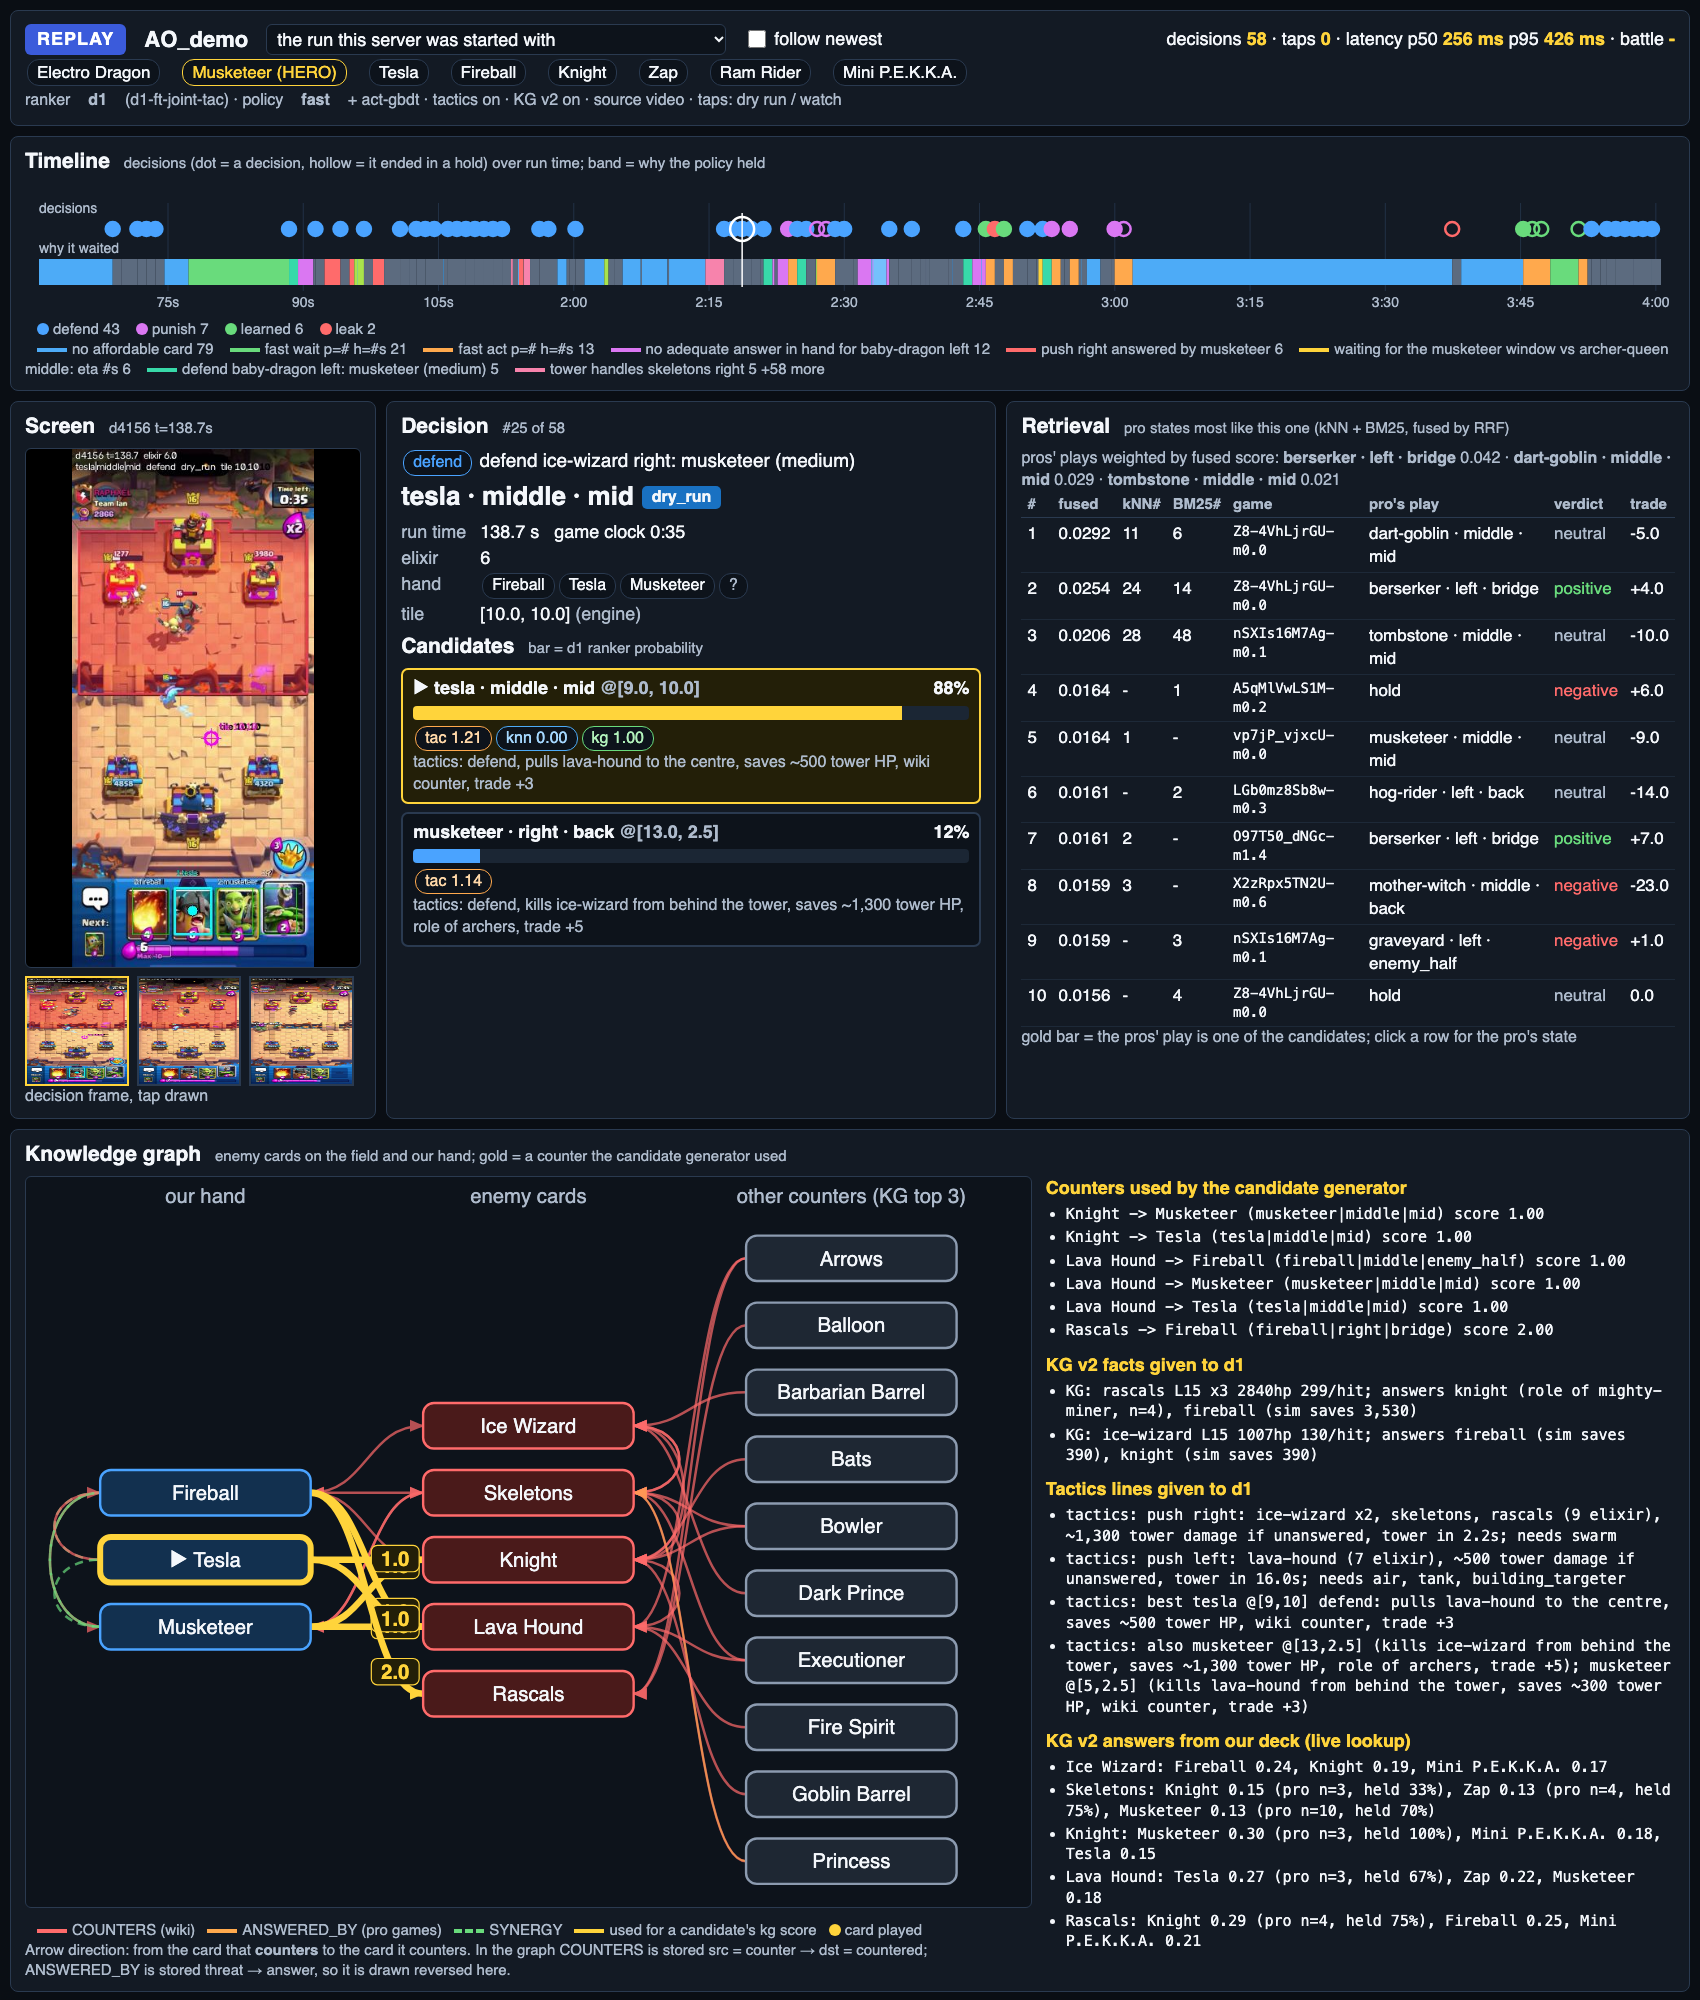
\includegraphics[width=\linewidth]{figs/dashboard.png}
\end{minipage}\hfill
\begin{minipage}[c]{0.37\columnwidth}
\captionsetup{justification=raggedright,singlelinecheck=false}
\caption{Decision dashboard on a video dry run. Top: timeline of decisions and hold reasons. Middle: decision frame; two candidates with d1 probabilities (Tesla 88\%) and the engine, kNN and KG scores behind them; the ten pro states retrieved by kNN+BM25 with RRF. Bottom: KG subgraph (our hand, enemy cards, counters used) and the \tw{KG:} and \tw{tactics:} lines d1 read.}
\label{fig:dashboard}
\end{minipage}
\end{figure}
